\documentclass[10pt,a4paper]{article}

% Language setting
% Replace `english' with e.g. `spanish' to change the document language
\usepackage[english]{babel}

% Set page size and margins
% Replace `letterpaper' with `a4paper' for UK/EU standard size
\usepackage[letterpaper,top=2cm,bottom=2cm,left=3cm,right=3cm,marginparwidth=1.75cm]{geometry}

% Useful packages
\usepackage{amsmath}
\usepackage{graphicx}
\usepackage{url}
\usepackage{float}
\usepackage{siunitx}
\usepackage{booktabs}
\usepackage[colorlinks=true, allcolors=black]{hyperref}
% column spacing and edge width
\geometry{margin=1.8cm}
\setlength{\columnsep}{0.7cm}

\begin{document}
	\twocolumn[
	\title{Performance Comparison of Single- and Dual-Camera Setups for Image-Based Satellite Orbit Determination}
	\author{Frederic Heil \\
		\texttt{frederic.heil@hs-weingarten.de}\\
		\textbf{Ravensburg-Weingarten University of Applied Sciences} \\
	}
	
	\maketitle
	
	\begin{abstract}
		\centering
		sss
	\end{abstract}
	\vspace{4em}
	]
	
	\section{Introduction}\label{sec:introduction}
	asdas
	\section{Methods}\label{sec:methods}
	\subsection{Single-Camera orbit determination}\label{sec:one_camera_determination}
	\subsubsection{Gaussian Method}\label{sec:gauss_method}
	The Gaussian method's approach is to numerically fit observations to a physically feasible orbit.
	The algorithm yields parameters for full orbit characterization, namely semi major axis $a$, eccentricity $e$, argument of periapsis $\omega$ and plane normal vector $n$.\newline A single observer camera is required, whereas three measurements each consisting of position vector $p_i$, view vector $v_i$ and corresponding timestamp $t_i$ need to be recorded to determine a solution. \cite{curtis_gauss_algo}
	\subsubsection{Simplified Gaussian Method}\label{sec:simplified_gauss_method}
	The simplified Gaussian method is a self developed approach to numerically fit observations to a physically feasibly circular orbit. Its incentive stems from the condition that satellite orbits low above earth's surface possess very low eccentricities and can mostly be considered circular. The algorithm yields parameters for circle-orbit characterization, namely semi major axis $a$ and plane normal vector $n$. \newline Similar to the Gaussian method, a single observer camera is required, whereas only two measurements each consisting of position vector $p_i$, view vector $v_i$ and corresponding timestamp $t_i$ need to be recorded to determine a solution. Hereby, the solution consists of two scalar parameters $\rho_1$ and $\rho_2$ which must satisfy the radius equality condition as well as the arc of a circle condition stated as follows:
	
	\begin{equation}
		\label{circle_gauss_circle_condition}
		|r_1|=|r_2|\Leftrightarrow \sqrt{(p_1+\rho_1v_1)^2}=\sqrt{(p_2+\rho_2v_2)^2}
	\end{equation}

	
	\begin{equation}
		\label{circle_gauss_time_condition}
		\begin{aligned}
			&\arccos\left(\frac{(p_1+\rho_1v_1)\cdot (p_2+\rho_2v_2)}{|(p_1+\rho_1v_1)|^2}\right)\cdot|(p_1+\rho_1v_1)|^{\frac{3}{2}}=\\
			&(t_2-t_1)\sqrt{\mu}
		\end{aligned}
	\end{equation}
	\cite{orbit_determination_preliminary}
	
	\subsection{Two camera trajectory determination}\label{sec:two_camera_determination}
	\subsubsection{Full parametric trajectory}\label{sec:full_parametric_trajectory}
	An orbital trajectory can be described as parametric curve lying in its orbital plane as follows: 
	\begin{equation}
		r(\theta)=\frac{a(1-e^2)}{1+e\cdot\cos(\theta-\omega)} \cdot \begin{pmatrix}
			\cos(\theta) \\
			\sin(\theta)
		\end{pmatrix}
	\end{equation}
	\noindent
	Given three positions in polar coordinates defined by radii $r_i$ and arguments $\theta_i$, the orbital properties $a$, $e$ and $\omega$ for eccentricities $e\neq 1$ and $e\neq 0$ are determined by:
	
	\begin{equation}
		\omega=\alpha_{13}-\arctan(G)
	\end{equation}
	\begin{equation}
		e=\frac{r_1-r_2}{C_{12}\cdot\cos(\alpha_{12}-\omega)}
	\end{equation}
	\begin{equation}
		a=\frac{r_1(1+e\cdot\cos(\theta_1-\omega))}{1-e^2}
	\end{equation}
	\noindent
	Hereby, $G$, $C_{12}$, $\alpha_{12}$ and $\alpha_{13}$ represent terms consisting of $r_1$, $r_2$, $r_3$, $\theta_1$, $\theta_2$ and $\theta_3$.\newline
	Two observer cameras are required, utilizing means of stereo vision. Three position vectors of the satellite are obtained by three synchronous measurements which yield values for radii $r_i$, arguments $\theta_i$ and the plane normal vector $n$. \cite{orbit_determination_preliminary}

	\subsubsection{Circular trajectory}\label{sec:circular_parametric_trajectory}
	This method once again simplifies the orbit to a circular trajectory. Two observer cameras are required, utilizing means of stereo vision. Two position vectors of the satellite are obtained by two synchronous measurements which yield the semi major axis $a$ and the plane normal vector $n$. \cite{orbit_determination_preliminary}
	
	\subsection{Experimental setups}
	\subsubsection{Variable observation spans and \\ observer placement}\label{sec:observation_setup}
	The goal is to create a measurement setup which can generate data sets usable by all presented single- and dual-camera orbit determination models to evaluate performance under different circumstances. All measurement data is captured from the  simulation \emph{Space Engine}, which makes the data synthetic. Space Engine is a software that incorporates a virtual universe including the solar system and nearby, real stars among other things \cite{space_engine}.\newline
	Identical virtual cameras are used in all observer locations and generate rectilinear images with the following properties:
	\begin{table}[H]
		\centering
		\begin{tabular}{l|r}
			Image Property & Value \\\hline
			Image frame [pixels] & 1000 x 1000 \\
			Field of view [°] & 17 x 17
		\end{tabular}
		\caption{\label{tab:sun_cam}Image properties of each observer camera}
	\end{table}
	\noindent
	In addition, several cameras are placed in strategic locations, so that  orbit determination can be performed subject to variable properties.

	\begin{figure}[H]
		\centering
		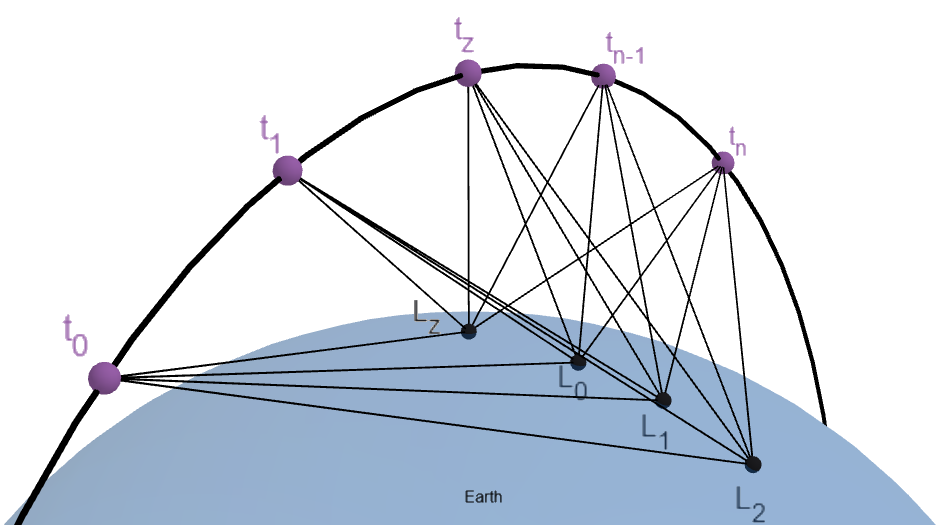
\includegraphics[width=1.0\linewidth]{images/observation_schematic.png}
		\caption{Schematic of strategic camera placement}
		\label{fig:observation_schematic}
	\end{figure}
	\noindent
	The schematic figure above shows the figurative placement of cameras as well as the planned synchronous recording of images. Starting at timestamp $t_0$ and proceeding with a fixed time interval, each camera takes a picture of the satellite at every time stamp until $t_n$. 
	For each timestamp from $t_0$ until $t_n$ and for each observer camera, position vector $p_i$ and view vector $v_i$ are recorded with the Earth Centered Inertial (ECI) coordinate system as reference frame.
	\newline
	As single- and dual-camera orbit determination methods for full determination require only three measurements each and for circular methods only two measurements respectively, we gain some modifiable parameters, which can be altered to observe changes in performance and accuracy of the models.\newline
	The first one, which is applicable to single- and dual-camera methods, being the alteration of observation time span $\Delta t$ which translates to the angular passage $\Delta \theta$ which the satellite passes in its orbit.\newline
	Secondly, applicable to dual-camera methods, is the variation in distance between two observer cameras which translates to a variable angle between intersecting lines of sight in the context of stereo vision. Consequently, the observer cameras are placed in the following locations on planet Earth within the simulation software:
	
	
	\begin{table}[htbp]
		\centering
		\begin{tabular}{llll}
			\toprule
			Location & Latitude & Longitude & Altitude \\
			\midrule
			$L_z$ & $-27.257356^\circ$ & $-64.963269^\circ$ & 313 m \\
			$L_0$ & $-27.301281^\circ$ & $-63.939256^\circ$ & 157 m \\
			$L_1$ & $-27.339896^\circ$ & $-63.847839^\circ$ & 153 m \\
			$L_2$ & $-27.378452^\circ$ & $-63.756358^\circ$ & 155 m \\
			$L_3$ & $-27.455384^\circ$ & $-63.573205^\circ$ & 149 m \\
			$L_4$ & $-27.608528^\circ$ & $-63.206133^\circ$ & 143 m \\
			$L_5$ & $-27.911902^\circ$ & $-62.468913^\circ$ & 127 m \\
			$L_6$ & $-28.506740^\circ$ & $-60.982091^\circ$ & 64 m \\
			$L_7$ & $-29.646743^\circ$ & $-57.958463^\circ$ & 64 m \\
			\bottomrule
		\end{tabular}
		\caption{Observation locations}
		\label{tab:observation_locations}
	\end{table}
	\noindent
	Hereby, it must be noted that given altitude values may deviate from real ones because these were measured within the simulation software. Cameras in locations from $L_0$ to $L_7$ are placed in a straight line, whereas the distance on the ground between location $L_i$ and $L_0$ doubles for each further location. The distance between $L_1$ and $L_0$ equates to 10km, between $L_2$ and $L_0$ to 20km and so on up until the distance between $L_7$ and $L_0$ equating to 640km. The purpose of location $L_z$ is to observe the satellite passing in the observer's zenith at timestamp $t_z$. It is not located on line $L_0L_7$.\newline
	Thirdly, applicable to single-camera methods, is the variation in distance to the orbital plane. Excluding special cases, the distance between observer locations and the orbital plane is constantly changing due to Earth's rotation. However, if the satellite is traversing quick enough from the observer's perspective, an average distance value can be used.
	Then, a ground truth orbit must be defined, applicable to all presented orbit determination models with the following properties:
	\begin{table}[H]
		\centering
		\begin{tabular}{l|r}
			Ground Truth Orbit Property & Value \\\hline
			Semi major axis [km] & 7067.445 \\
			Eccentricity & 0 \\
			Inclination [°] & 52 \\
			Ascending Node [°] & 0 \\
			Reference epoch & J2000 \\
			Initial mean anomaly $\theta_0$ [°] & 0
		\end{tabular}
		\caption{Ground truth orbit properties}
		\label{tab:ground_truth_orbit}
	\end{table}
	\noindent
	Consequently, the orbit should be circular. It is tilted against the equatorial, whereat the plane normal vector derives from \emph{inclination} and \emph{ascending node} as $n=(0.0, -0.78801075, 0.61566148)$.\newline
	Furthermore, it is noted that location $L_z$ was chosen for the predefined timestamp $t_z = \text{2000.01.01 20:03:00}$ [UT], so that the satellite passes in the observer's zenith with given ground truth properties.
	
	\subsection{Influence of star-based \\ view vector determination}
	As elaborated in the preliminary text, view vector determination relies three known stars or rather their view vectors $v_{S1}$, $v_{S2}$ and $v_{S3}$ to form a matrix $M$ for triangulation \cite{orbit_determination_preliminary} which is more or less suited for view vector determination through triangulation. One metric to measure suitability is the determinant $d$ as it indicates linear dependency of its row/column vectors formulated as follows:
	\begin{equation}\label{eq:determinant}
		d = \det(M)
	\end{equation} 
	\noindent
	Another useful metric is the condition number $\kappa(M)$ which indicates how sensitive the triangulation matrix $M$ is to errors formulated as follows:
	\begin{equation}
		\begin{aligned}
			\kappa(M) = \left\lVert M \right\rVert_2 \cdot \left\lVert M^{-1}\right\rVert_2 \text{with}\quad \left\lVert M \right\rVert_2 = \max_k \sigma_k
		\end{aligned}
	\end{equation}
	\noindent
	Hereby, the 2-norm of matrix $M$ is defined by its maximum singular value $\sigma_k$ \cite{condition_numbers}.\newline
	We hypothesize that there might be a correlation between the accuracy of a predicted orbit and the suitability of matrix $M$ used for view vector determination. For testing purposes, we perform orbit determination of the ground truth orbit defined in \ref{tab:ground_truth_orbit} using distinct sets of stars for view vector calibration. Observations are conducted by one camera placed at $L_5$ starting at certain predefined time stamps so that numerous background stars are visible to form many distinctive 
	sets of stars for calibration. The determination algorithm of choice is the simplified Gaussian method with a fixed observation span $\Delta t = 7s$.
	
	\subsubsection{Influence of variable Semi Major Axis}
	The goal of this setup to verify whether the self developed simplified Gaussian method holds under differing conditions, specifically with varied semi major axis. Other experiments use solely the ground truth orbit defined in table \ref{tab:ground_truth_orbit}. This experiment modifies the orbit's semi major axis and initial mean anomaly $\theta_0$ so that the satellite always passes in the zenith of $L_z$ and $t_z$ which makes it easily visible from all observer locations. The semi major axis is chosen in such a way that the range of mean altitudes cover the entire range of the Low Earth Orbit as follows:
	
	\begin{table}[H]
		\centering
		\begin{tabular}{ccc}
			\hline
			Semi major axis & Mean altitude & $\theta_0$ \\
			\hline
			6667.445 km & 300 km  & 198.86° \\
			6867.445 km & 500 km  & 282.36° \\
			7067.445 km & 700 km  & 0.00° \\
			7267.445 km & 900 km  & 72.33° \\
			7467.445 km & 1100 km & 139.85° \\
			7667.445 km & 1300 km & 203.00° \\
			7867.445 km & 1500 km & 262.16° \\
			8067.445 km & 1700 km & 317.67° \\
			8267.445 km & 1900 km & 9.85° \\
			8467.445 km & 2100 km & 58.97° \\
			\hline
		\end{tabular}
		\caption{Modified properties of ground truth orbit}
		\label{tab:modified_satellite_altitude}
	\end{table}
	\noindent
	Once again, observations are conducted by one camera placed at $L_5$ with a fixed observation span $\Delta t = 7s$.
	
	\subsection{Metrics}
	\subsubsection{Parameter stability}\label{sec:param_stability_definition}
	All presented orbit determination methods yield values for semi major axis $a$ and plane normal vector $n$. Additionally, methods not assuming a circular orbit, yield values for eccentricity $e$ and argument of periapsis $\omega$. The goal is to compare measured (denoted $m$) with ground truth (denoted $g$) properties in a generalized form independent of units. For this reason, we define error metrics $f_a$, $f_e$, $f_{\omega}$ and $f_n$ for $a$, $e$, $\omega$ and $n$ as follows::\newline
	\begin{equation}\label{eq:error_sma}
		f_a=\frac{|a_g-a_m|}{a_g}
	\end{equation}
	\begin{equation}\label{eq:error_ecc}
		f_e=|e_g-e_m|
	\end{equation}
	\begin{equation}\label{eq:error_omega}
		f_\omega=|\omega_g-\omega_m|
	\end{equation}
	\begin{equation}\label{eq:error_n}
		f_n=\arccos\left(\frac{n_g\cdot n_m}{|n_g|\cdot|n_m|}\right)=\arccos(n_g\cdot n_m) \\
	\end{equation}
	Hereby, specifically for metric \ref{eq:error_omega}, it must be noted that this expression is undefined if ground truth or measured orbit has an eccentricity of $e=0$.
	
	\subsubsection{Propagation error}\label{sec:error_propagation_definition}
	The determined orbit of a satellite differs from the actual ground truth by a margin of error. As the satellite continues orbiting Earth, actual and predicted position continue drifting apart due to this error. Carpenter et al. state that the position error along the trajectory arises from the semi major axis error .This formulates as an equation for the variation in orbital period $\delta T$ subject to variation in semi major axis $\delta a$ as:
	
	\begin{equation}
		\delta T = 3\pi\sqrt{\frac{a}{\mu}}\cdot\delta a
	\end{equation}
	\noindent
	\cite{semi_major_axis_knowledge} \newline
	Our approach is to formulate the position or rather propagation error in such a way that factors in all orbital parameters
	The previous section quantifies the error of individual properties. 
	\section{Results and Discussion}\label{sec:results_discussion}
	\subsection{Parameter error}\label{sec:param_stability_result}
	\subsection{Error propagation}\label{sec:error_propagation_result}
	\subsection{Lower altitude bound for feasible \\ trajectory determination}\label{sec:lower_bound}
	\subsection{Stability of circular models applied to elliptical orbits}\label{sec:stability_circular}
	\section{Conclusion}\label{sec:conclusion}
	
	\onecolumn
	\begin{thebibliography}{9}
		\setlength{\itemsep}{4pt}       % space between bibliography items
		\setlength{\parskip}{0pt}       % space between paragraphs
		\setlength{\parsep}{0pt}        % extra space within items
		
		\bibitem{curtis_gauss_algo} Curtis, H.D. (2010): \emph{Gauss method of preliminary orbit determination}. In: \emph{Orbital Mechanics for Engineering Students}, 2nd ed., pp. 297--304. \newline \url{https://shop.elsevier.com/books/orbital-mechanics-for-engineering-students/curtis/978-0-12-374778-5} \newline Accessed: 2026-05-03 
		
		\bibitem{orbit_determination_preliminary} Heil, F. (2026): \emph{Image based trajectory determination of artificial satellites}. \newline \url{https://github.com/stonkchonk/satellite-trajectories/blob/main/thesis/preliminary.pdf} \newline Accessed: 2026-09-29 
		
		\bibitem{space_engine} Cosmographic Software LLC (2026): \emph{About}. SpaceEngine. \newline \url{https://spaceengine.org/manual/making-addons/scenario-scripts/} \newline Accessed: 2026-09-29 
		
		\bibitem{condition_numbers} University of Illinois Urbana-Champaign (n.d.): \emph{Condition Numbers}. CS 357 Textbook. \newline \url{https://cs357.cs.illinois.edu/textbook/notes/condition.html} \newline Accessed: 2026-10-08
		
		\bibitem{semi_major_axis_knowledge}
		Carpenter, J.R. and Schiesser, E.R. (2001):
		\emph{Semi-Major Axis Knowledge and GPS Orbit Determination}.
		In: \emph{Journal of the Institute of Navigation}, 48(1).
		\newline
		\url{https://ntrs.nasa.gov/citations/20000084327}
		\newline
		Accessed: 2026-10-09
	\end{thebibliography}
\end{document}